\section{Logistic Regression}

    \subsection{Classification}
        
        \begin{itemize}
            \item Binary Classification: y $\in \{0, 1\}$, where 0 denotes the negative class; 1 denotes the positive class.
            \item Multi-class Classification:y $\in \{0, 1, \cdots, n\}$ 
        \end{itemize}

        We will be using binary classification: 
        \begin{itemize}
            \item Linear regression is not suitable for classification: since $h_\theta (x)$ can output out of range, i.e. $<0$ or $>1$. 
            \item We will use \textbf{logistic regression}, which ensures that the output $h_\theta (x)$ is between 0 and 1.
        \end{itemize}

    \subsection{Hypothesis Representation}

        \subsubsection{Logistic function}
            The idea is to have $ 0 \leq h_\theta (x) \leq 1$. Instead of the linear regression hypothesis: $h_\theta (x) = \theta^T x$, we will let:
                \[
                    h_\theta (x) = g (\theta^t x)
                ,\]

                where \[
                    g(z) = \frac{1}{1+e^{-z}}
                \]

                g(z) is known as the \textbf{logistic function}, also known as the Sigmoid function. Figure \ref{fig:sigmoid-function} shows a plot of the logistic function, which ranges from 0 to 1. 


                which yields 
                \begin{equation}
                    h_\theta (x) = \frac{1}{1+e^{-z}}
                    \label{eq:log-reg-hypo}
                \end{equation}


                \begin{figure}[htbp]
                    \centering
                    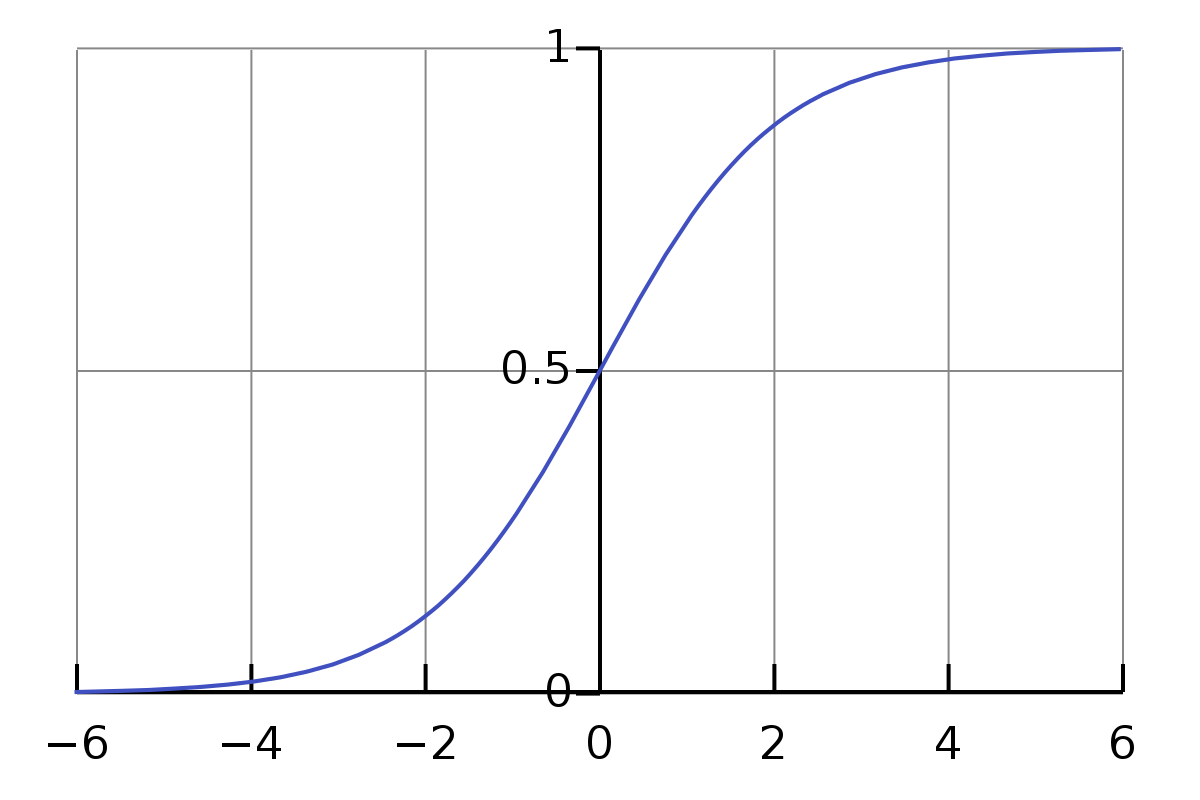
\includegraphics[width=0.5\textwidth]{image/sigmoid-function.png}
                    \caption{Sigmoid Function}
                    \label{fig:sigmoid-function}
                \end{figure}


        \subsubsection{Interpretation of Hypothesis Output}
        $ h_\theta (x)= $ estimated probability that y= 1 on input x. For example, $h_\theta(x)= 0.7$ gives us a probability of 70\% that are output is 1. 
        From a probability theory point of view, one can express $h_\theta (x)$ as $ P(y=1 \mid x;\theta)$. 

        Note that since this is a probability and the total probability sums up to 1, and the real y can only be either 0 or 1:
        \[
            P(y=0 \mid x; \theta) + P(y=1 \mid x;\theta) = 1
        \] 
            


    \subsection{Decision Boundary}

    Recall so far we have $h_\theta (x) = g(\theta^T x)$ and $g(z) = \frac{1}{1+exp(-z)}$. Suppose we set $h_\theta(x) = 0.5$ to be our determining factor for whether y= 0 or y =1. Note that from \ref{fig:sigmoid-function}, one can observe that $h_\theta(x) = 0.5$ corresponds to $\theta^T x = 0$, which is the \textbf{decision boundary}. The decision boundary is the equation which separates the different classes on a plot. There are linear and non-linear decision boundaries.


    \subsection{Cost function}

        Previously, we had $ J(\theta) = \frac{1}{m} \sum_{i=1}^{m} Cost( h_\theta ( x^{(i)}), y^{(i)} )$, where $Cost (h_\theta(x), y) = \frac{1}{2} (h_\theta(x) - y)^2$. 
        Now, the definition of the hypothesis $h_\theta$ has changed to $\frac{1}{1+exp(-\theta^T x}$, as a result the cost function is now non-convex. \\ 
        
            \textbf{Logistic Regression Cost Function}

            Therefore, a new cost function definition is needed. We propose: 

            \[
                Cost (h_\theta(x), y) = 
                \begin{cases}
                    -log(h_\theta(x))       &\quad \text{if } y=1 \\
                    -log(1- h_\theta(x))    &\quad \text{if } y=0 \\
                \end{cases}
            \] 

            Note that Cost=0, if y=1, $h_\theta(x) =1$; but as $h_\theta(x) \to 0$, then $Cost \to \infty$. This proposition captures the intuition that if $h_\theta(x)=0$, predict $P(y=1 \mid x;\theta)$, but y ends up being 1, we will penalize the learning algorithm by very large cost.
            
    \subsection{Simplified Cost Function and Gradient Descent}
        

            Since y can only be either 0 or 1, we can simplify the cost function.
       

            \begin{equation}
                \begin{split}
                    J(\theta)   &= \frac{1}{m}\, \sum_{i=1}^{m}\, Cost\,(\, h_\theta ( x^{(i)})\, ,\, y^{(i)} ) \\
                    &= \frac{-1}{m} \, [ \; \sum_{i=1}^{m}\, y^{(i)}\, log\, h_\theta (x^{(i)})\; +\; (1-y^{(i)})\: log\:(\,1-h_\theta(x^{(i)})\,) \;] 
                \end{split}
                \label{eq:simplified-cost-function}
            \end{equation}
            Equation \ref{eq:simplified-cost-function} is based on Maximum Likelihood Estimation.


            A vectorized implementation is, for a design matrix $\mathbf{X}$:
            \begin{equation}
                \boxed{
                    h = g(\mathbf{X\theta})
                }
                \label{eq:vectorized-logistic-hypothesis}
            \end{equation} 

            
            \begin{equation}
                \boxed{
                    J (\theta) = \frac{1}{m} (-y^T log(h) - (1-y)^T log(1-h) )
                }
                \label{eq:vectorized-logistic-cost-function}
            \end{equation} \\

            
            For gradient descent,we would want to $\min_{\theta} J(\theta)$:\\ 
             Repeat \{
                \[ \theta_j := \theta_j - \alpha \frac{\partial }{\partial \theta_j} J(\theta)\] \}\\

   
            We can compute the partial derivative of $J(\theta)$, which is identical to that of linear regression:
            \[
                \frac{\partial }{\partial \theta_j} J(\theta) = \frac{1}{m} \sum_{i=1}^{m} ( h_\theta (x^{(i)}) - y^{(i)} )\cdot x^{(i)} 
            \]\\
            However, in this case the hypothesis function $h_\theta(x) = \frac{1}{1+exp(-\theta^T x}$ has changed!

            A vectorized implementation for this is:
            \begin{equation}
                \boxed{
                    \mathbf{\theta} := \mathbf{\theta} - \frac{\alpha}{m} \mathbf{X}^T( g (\mathbf{X\theta}) - \mathbf{y}))
                }
                \label{eq:vectorized-logistic-gradient-decent}
            \end{equation}



    \subsection{Advanced Optimization}
        \subsubsection{Taking a Step Back}
            If we take a step back, and consider essentially what tasks we are performing. We need to compute two things:
            \begin{enumerate}
                \item $J(\theta)$
                \item $\frac{\partial}{\partial \theta_j}J(\theta)$
            \end{enumerate}

        \subsubsection{Optimization Algorithm}
        There exists other more sophisticated and faster ways to optimize $\theta$ instead of gradient descent; they often do not involve selecting learning rate $\alpha$ and are more efficient. However, these algorithms are harder to code by hand. It is suggested that we use libraries for such algorithms. 

        We can write a single function that returns both  $J(\theta)$ (jVal) and  $\frac{\partial}{\partial \theta_j}J(\theta)$ (gradient):

        \begin{lstlisting}
        function [jVal, gradient] = costFunction(theta)
            jVal = [...code to compute J(theta)...];
            gradient = [...code to compute derivative of J(theta)...];
        end
            
        \end{lstlisting}

        Then we can use octave's "fminunc()" optimization algorithm along with the "optimset()" function that creates an object containing the options we want to send to "fminunc()".

        \begin{lstlisting}
            options = optimset('GradObj', 'on', 'MaxIter', 100);
            initialTheta = zeros(2,1);
            [optTheta, functionVal, exitFlag] = fminunc(@costFunction, initialTheta, options);
            
        \end{lstlisting}
        

        We then give to the function "fminunc()" our cost function, our initial vector of theta values, and the "options" object that we created beforehand.
        \subsection{Multiclass Classification: One-vs-All}
            Now, let's extend the binary classification of data to multi-classes, i.e expanding our definition of y s.t. y=\{0, 1, \ldots, n\}.
            We will divide out problem into n+1 (0\ldots n) binary classification problems. In each problem, we predict the probability that y is a memember of one of our class. We train a logistic regression classifier $h_\theta ^{(i)} (x) $ $\forall$ i to predict y = i:
            \begin{equation}
                h_\theta^{(i)} (x) = P (y=i \mid x;\theta)
                \label{eq:multiclass-logistic-classifier}
            \end{equation}

            Figure \ref{fig:multi-class-regression} shows an example of the procedure of classifying three classes. We choose one class and then lump all the others into a single second class (hence the name One-vs-All). We apply the binary logisic regression repeatedly and use the hypothesis that returns the highest value. 

            \begin{equation}
                prediction\,=\: \max_{i}\: (\, h_\theta ^{(i)} (x) \,)   
                \label{eq:max-log-regre}
            \end{equation}
            

            \begin{figure}[htbp]
                \centering
                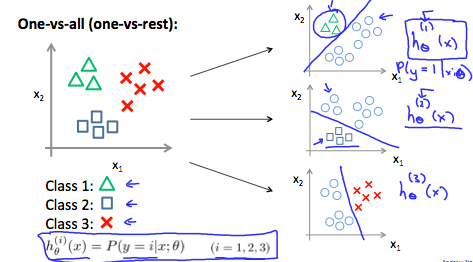
\includegraphics[width=\textwidth]{image/multi-class.png}
                \caption{Example of Multiclass Logistic Regression}
                \label{fig:multi-class-regression}
            \end{figure}
